% !TEX root = ../main.tex

\chapter{相干首波}

\section{声速的测量}

任何合格的物理本科生都熟悉如何在空气或水中测量声速,如共振波节法、相位法、时差法。前两者的原理都是寻找信号某个相位下的空间位置,从而通过逐差法确定声波的波长;后者则是考虑到了声学探头中压电陶瓷进行声-电转换所需要的固有时间,因此通过求空间位置与到达时间的斜率以确定声速。事实上,在颗粒固体中测量声速时,这些方法都有不同程度的应用,如 Paul A.Johnson 和 Xiaoping Jia 同时使用共振法与行波法(即飞行时间法,Time of Flight,T.O.F.)测定颗粒介质中的声速\cite{Johnson_2005};而在地震学中,基于连续小波变换(Continuous Wavelet Transform, CWT)和频散能量图求解地震波相速度的方法也被广泛应用。本节将介绍如何使用飞行时间法与频散能量图测量颗粒介质中的声速。

\subsection{装置搭建}



\subsection{飞行时间法}

飞行时间法测定声速的原理即测量试探声波从声源探头到接收探头的时间差 $\Delta t$,但如何定义声波的到达时间(Arrival Time)是值得商榷的问题。Ellák Somfai 等人尝试定义颗粒介质中声波的三个不同的到达时间:波前到达时间 $t_{0}$(由于噪声的存在,波前通常被定义为上升沿峰值 $A_{1}$ 的 $\num{10}\%$ 处,部分更激进的研究者会选取为 $3\%$),波峰到达时间 $t_{1}$,首次过零时间 $t_{2}$\cite{PhysRevE.72.021301}。良好定义的波速应当满足在不同厚度下测得的结果相近。

\subsubsection{信号最佳参考点选取}

由于使用的 Tektronix 示波器对源信号与响应信号进行了同步采集,因此容易确定具体的到达时间。基于调整噪声阈值、最小半高宽等参数的寻峰算法,我们可以准确确定源信号的峰值,从而根据因果关系筛去可能错误识别的噪声。下图是对典型的响应信号进行三种不同到达时间的识别结果。

% \begin{figure}[!hbtp]
%   \centering
%   \subcaptionbox{健康/损伤信号}%
%                 [7cm]{\includegraphics[height=6cm]{figures/signal_1.png}}
%   \hspace{1cm}
%   \subcaptionbox{散射信号}%
%                 [7cm]{\includegraphics[height=6cm]{figures/signal_2.png}}
%   \caption{响应信号处理}
%   \label{fig:bisubcaptionbox}
% \end{figure}

\subsection{频散能量图法}

\subsubsection{测量相速度的原理推导}

如果我们将颗粒介质中的声学传播简单考虑为单频球面波,即

\begin{equation}
  s(x,t) = A_{0}{\ee}^{-\alpha x}{\ee}^{\ii(\omega x/V_{\varphi}-\omega t)},
  \label{eq:spherical_wave}
\end{equation}

考虑在距离声源 $x_{1}$ 与 $x_{2}$ 处的两个接收探头,分别接收到声波信号 $S_{1}(t)$ 与 $S_{2}(t)$。则能求解相速度为

\begin{equation}
  V_{\varphi} = \frac{x_{2}-x_{1}}{\Delta \varphi}\omega.
\end{equation}

我们很容易想到通过 FFT 算法求解两次信号的相位频谱 $\varphi_{i}(\omega)$, 但是显然

\begin{equation}
  \Delta \varphi = \varphi_{2}(\omega) - \varphi_{1}(\omega) + 2N(\omega)\uppi
\end{equation}

对于 $N(\omega)$ 的确定则较为困难,因此地震学提出使用频散能量图观察相速度可能的分布情况。

引入互关联函数 $C_{i,j}(\tau)$:

\begin{equation}
  C_{i,j}(\tau) = \int_{-\infty}^{+\infty}S_{i}(t)S_{j}(t+\tau)\mathrm{d}t.
\end{equation}

其中 $\tau$ 是描述信号延迟时间的参数。该函数是一个时域函数,对其进行傅里叶变换:

\begin{align}
  \mathcal{F}[C_{1,2}(\tau)] &= \frac{1}{2\uppi}\int_{-\infty}^{+\infty}{\ee}^{-\ii\omega\tau}\int_{-\infty}^{+\infty}S_{1}(t)S_{2}(t+\tau)\mathrm{d}t\mathrm{d}\tau \nonumber \\
  &= \frac{1}{2\uppi}\int_{-\infty}^{+\infty}S_{1}(t)\int_{-\infty}^{+\infty}{\ee}^{-\ii\omega\tau}S_{2}(t+\tau)\mathrm{d}\tau\mathrm{d}t \nonumber \\
  &= \int_{-\infty}^{+\infty}S_{1}(t)S_{2}(\omega){\ee}^{\ii\omega t}\mathrm{d}t \nonumber \\
  &= 2\uppi S_{1}^{*}(\omega)S_{2}(\omega).
\end{align}

通过狄拉克函数 $\delta(\omega-\omega_{n})$ 提取信号分量 $\omega_{n}$ 的延迟时间的信息,再对其进行逆傅里叶变换:

\begin{align}
  \mathcal{F}^{-1}\left\{\delta(\omega-\omega_{n})\mathcal{F}[C_{1,2}(\tau)]\right\} &= \int_{-\infty}^{+\infty}2\uppi S_{1}^{*}(\omega)S_{2}(\omega)\delta(\omega_{n}){\ee}^{\ii\omega\tau}\mathrm{d}\omega \nonumber \\
  &= 2\uppi S_{1}^{*}(\omega_{n})S_{2}(\omega_{n}){\ee}^{\ii\omega_{n}\tau}.
\end{align}

具体绘制时我们只需通过 $2\uppi S_{1}^{*}(\omega_{n})S_{2}(\omega_{n}){\ee}^{\ii\omega_{n}\tau}$ 最大值归一化后的实部即可。其物理含义是,延迟时间为 $\tau$ 时,即该频率分量 $\omega_{n}$ 对应的相速度为 $V_{\varphi} = \Delta x/\tau$ 的可能性大小,所以得到的将是 $[-1,1]$ 之间的数值。通过设置离散频率分布 $\{\omega_{n}\}$, 即可查看在颗粒介质中可能的相速度分布。需要说明的是,频散能量图没有从根本上解决 $N(\omega)$ 的确定问题,但是为辅助飞行时间法测定声速提供了更直观的参考工具。

\subsubsection{颗粒介质中相速度分布}


\begin{figure}[!hbtp]
  \centering
  \bisubcaptionbox{在 $x_1=1.1\unit{cm}$ 与 $x_{2}=2.0\unit{cm}$ 处采集的响应信号}{Reponse signal captured at $x_1=1.1\unit{cm}$ and $x_{2}=2.0\unit{cm}$}%
                [7cm]{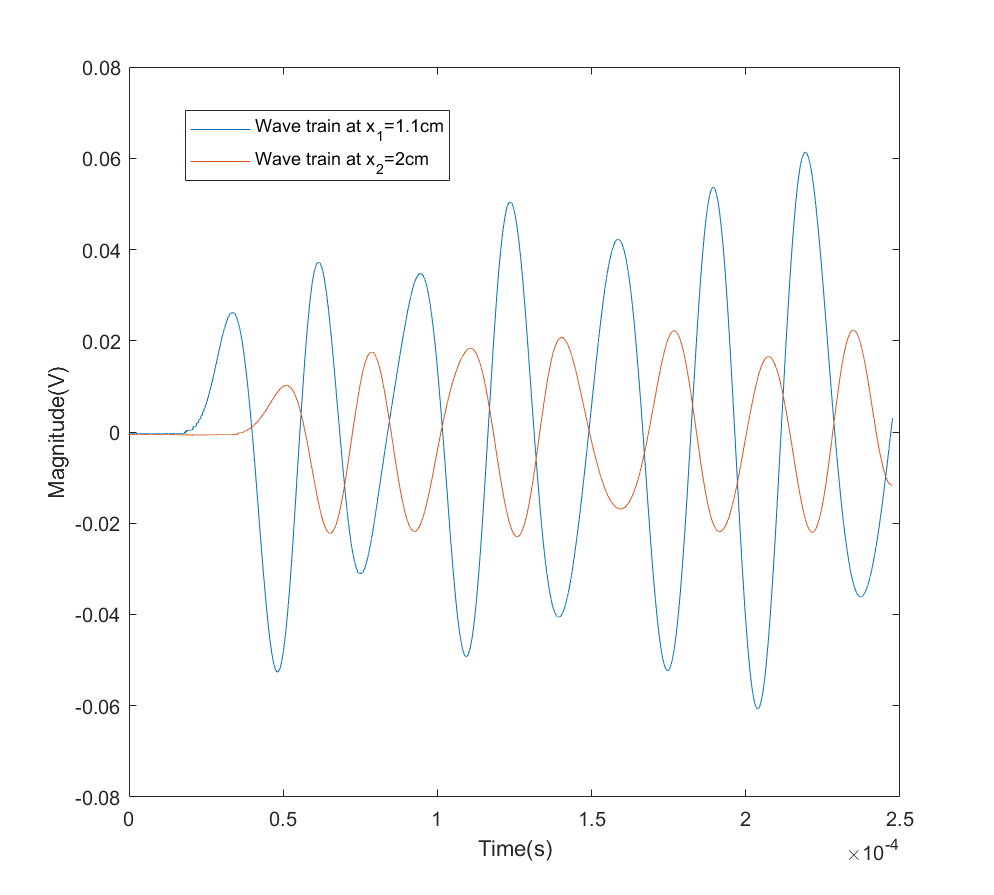
\includegraphics[height=6cm]{figures/2_wave_train.png}}
  \hspace{1cm}
  \bisubcaptionbox{$0-60\unit{kHz}$ 的相速度频域分布热图}{Phase velocity frequency distribution heat map at $0-60\unit{kHz}$}%
                [7cm]{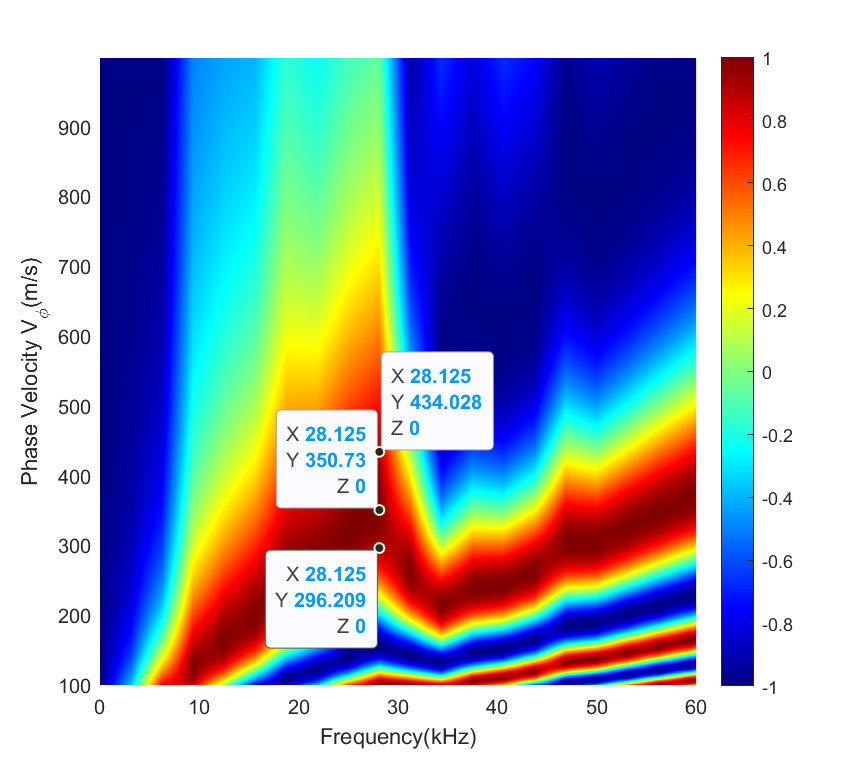
\includegraphics[height=6cm]{figures/2_cwt_v_phi.png}}
  \bicaption{根据异地响应信号计算频散能量图}{Dispersion energy map calculated from separated response signals}
  \label{fig:dispersion_energy}
\end{figure}

图 \ref{fig:dispersion_energy} 展示了在单轴应力容器中,根据不同采集距离下的两道压缩波信号绘制的频散能量图。可以看到两道信号在发射信号的中心频率 $f_{c} = 30\text{ kHz}$ 处的相速度约为 $V_{\varphi} = 350\pm 10\unit{m/s}$

\section{声速与单轴应力的指数关系}

\subsection{等效介质理论(EMT)}

\subsection{实验验证}

\section{超声脉冲在颗粒介质中的展宽}

颗粒介质通过异质性的力链网络传递应力,因此声波在颗粒介质中传播时会出现剧烈的畸变现象,其中脉冲波的展宽是较为明显的现象之一。本节讨论了颗粒介质厚度以及单轴应力大小对于脉冲波展宽的影响。

\subsection{归一化宽度的定义}

在信号处理中,常见的对于峰宽度的定义通常是半高宽;事实上,我们在处理响应信号的到达时间时,使用的寻峰算法中的参数就包含了半高宽阈值。但是在这里,我们引入的归一化宽度参数同时考虑了峰值与波前的位置:

\begin{equation}
  W \equiv \frac{t_{1}-t_{0}}{t_{1}},
\end{equation}

其中 $t_{0}$ 与 $t_{1}$ 分别为波前与峰值的到达时间。我们在测定最佳信号参考点的时候已经意识到,脉冲的展宽实际上已经在一定程度上反映了在颗粒介质中存在的色散关系;而峰值到达时间定义的飞行时间速度,即在试探信号中心频率附近,在距离上更具有稳定性。因此,通过与中心频率关联的 $t_{1}$ 来对信号进行缩放是合理的。我们还将在后文的讨论中通过数据处理进一步证明这一点。

\subsection{归一化宽度与颗粒介质厚度的关系}

\subsubsection{理论推导}

我们先从最简单的一维弹簧链开始推导。凝聚态物理中,我们已经知道一维晶格的色散关系为

\begin{equation}
  \omega=\sqrt{\frac{4C}{M}}\left|\sin\left(\frac{ka}{2}\right)\right|,
\end{equation}

其中 $C$ 为弹性系数,$M$ 为弹簧所连接质点的质量,$a$ 为质点间距/晶格常数。我们将其写为反函数形式:

\begin{equation}
  k(\omega) = \frac{2}{a}\arcsin{\left(\sqrt{\frac{M}{4C}}\omega\right)}.\label{eq:1D_dispersion_relation}
\end{equation}

在这里,我们对其应用长波极限 $ka\ll 1$, 从而求得波速度:

\begin{equation}
  V = \lim_{ka\ll 1}\frac{\omega}{k} = \sqrt{\frac{C}{M}}a.
\end{equation}

使用 $V$ 替换式~\eqref{eq:1D_dispersion_relation} 中的 $C$,$M$ 项,且假定长波极限下的声速 $V$ 充分大,使得我们足以通过麦克劳林级数将其展开至前两项:

\begin{equation}
  k = \frac{2}{a}\left[\frac{a\omega}{2V} + \frac{1}{6}\left(\frac{a\omega}{2V}\right)^{3} + o\left(\frac{1}{V^3}\right)\right]\approx\frac{\omega}{V} + \frac{2\omega^{3}a^{2}}{3V^{3}},
\end{equation}

将其代入至波数项中,我们将看到

\begin{equation}
  \text{exp}\left[{\ii \left(\frac{\omega}{V} + \frac{2a^{2}\omega^{3}}{3V^{3}}\right)x}\right] = \text{exp}[{\ii\omega t_{1}}]\text{exp}\left[{\ii\left(\frac{\omega}{\omega_{1}}\right)^{3}}\right],\quad t_{1} = \frac{x}{V},\quad \omega_{1} = \sqrt[3]{\frac{3V^{3}}{2a^{2}x}}.
\end{equation}

而我们已经知道,在傅里叶变换中,存在关系

\begin{align}
  \mathcal{F}[f(t+t_{1})] = \mathcal{F}[f(t)]{\ee}^{\ii\omega t_{1}},\label{eq:translation_property}\\
  \mathcal{F}[f(\omega_{1}t)] = \frac{1}{|\omega_{1}|}\hat{f}\left(\frac{\omega}{\omega_{1}}\right),\label{eq:scale_property}\\
  \mathcal{F}[\text{Ai}(t)] = \text{exp}\left[\ii\cdot \frac{1}{3}\omega^3\right].
\end{align}

将波数项代入至 $a(x,-t)$ 中,并对其进行傅里叶变换:

\begin{equation}
  \mathcal{F}[a(x,-t)] = \frac{1}{2\uppi}\int_{-\infty}^{+\infty}A_{0}{\ee}^{\ii\omega t_{1}}{\ee}^{\ii(\omega/\omega_{1})^{3}}e^{\ii\omega t}e^{-\ii\omega t}\mathrm{d}t = \frac{A_{0}}{2\uppi}{\ee}^{\ii\omega t_{1}}{\ee}^{\ii(\omega/\omega_{1})^{3}}.
\end{equation}

所以,根据傅里叶变换的平移性质~\eqref{eq:translation_property}与尺度性质~\eqref{eq:scale_property},我们得到源信号形式可近似为通过 $\omega_{1}$ 控制宽度的 Airy 函数:

\begin{equation}
  s(x,t) = \omega_{1}\text{Ai}\left[\omega_{1}(t_{1}-t)\right].
\end{equation}

因此,在一维弹簧链中,脉冲波传播到距离 $L$ 处的归一化宽度为

\begin{equation}
  W \approx \frac{\pi}{2\omega_{1}}\frac{1}{t_{1}}\propto L^{-2/3}.
\end{equation}

考虑一维球链时,使用 $a=2R$ 替换即可得到对应的公式\cite{PhysRevE.91.022205}。接下来我们进一步考虑颗粒介质中衰减项 $\alpha$ 的影响。

\subsubsection{实验验证}

\subsection{归一化宽度与单轴应力的关系}
